\usetikzlibrary{decorations.pathmorphing}

\begin{figure}[h!]
    \centering
    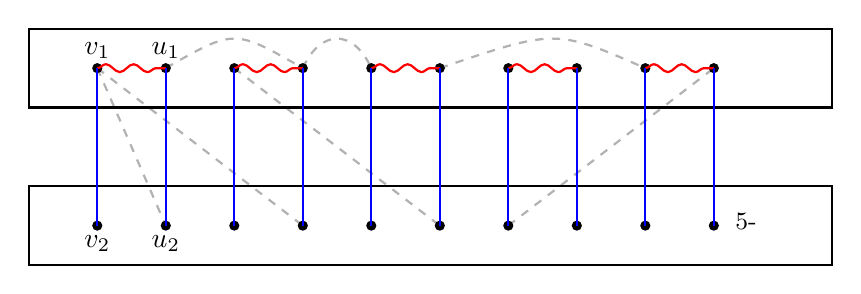
\begin{tikzpicture}[scale=0.5]     % Adjust the scale factor here
        % Scale factor for wider picture
        \pgfmathsetmacro{\scaleFactor}{1.2}

        % Define a lighter gray color
        \definecolor{lightergray}{gray}{0.7}

        % Draw a half-oval lighter gray dashed edge between vertex 2 and vertex 4 inside the rectangle
        \draw[lightergray, thick, dashed] (2.9 * \scaleFactor, 1) .. controls (4.35 * \scaleFactor, 2) and (4.35 * \scaleFactor, 2) .. (5.8 * \scaleFactor, 1);

        % Draw a half-oval lighter gray dashed edge between vertex 4 and vertex 5 inside the rectangle
        \draw[lightergray, thick, dashed] (5.8 * \scaleFactor, 1) .. controls (6.175 * \scaleFactor, 2) and (6.875 * \scaleFactor, 2) .. (7.25 * \scaleFactor, 1);

        % Draw a half-oval lighter gray dashed edge between vertex 6 and vertex 10 inside the rectangle
        \draw[lightergray, thick, dashed] (8.7 * \scaleFactor, 1) .. controls (11.15 * \scaleFactor, 2) and (11.15 * \scaleFactor, 2) .. (13.05 * \scaleFactor, 1);

        % Draw a straight lighter gray dashed edge between the first vertex in the top rectangle and the second vertex from the bottom
        \draw[lightergray, thick, dashed] ({1.45 * \scaleFactor}, 1) -- ({2.9 * \scaleFactor}, -3);

        % Draw a straight lighter gray dashed edge between the first vertex in the top rectangle and the fourth vertex from the bottom
        \draw[lightergray, thick, dashed] ({1.45 * \scaleFactor}, 1) -- ({5.8 * \scaleFactor}, -3);

        % Draw a straight lighter gray dashed edge between the 7th vertex from the bottom and the 10th vertex from the top
        \draw[lightergray, thick, dashed] ({10.15 * \scaleFactor}, -3) -- ({14.5 * \scaleFactor}, 1);

        % Draw a straight lighter gray dashed edge between the third vertex from the top and the sixth vertex from the bottom
        \draw[lightergray, thick, dashed] ({4.35 * \scaleFactor}, 1) -- ({8.7 * \scaleFactor}, -3);

        % Draw the first horizontal rectangle (20% wider)
        \draw[thick] (0,0) rectangle (17 * \scaleFactor, 2);

        % Draw the 10 vertices inside the first rectangle, sorted on a horizontal line, avoiding borders
        \foreach \i in {1,...,10} {
            \node[circle, fill, inner sep=1.3pt] at ({1.45 * \scaleFactor + 1.45 * \scaleFactor * (\i-1)}, 1) {};
        }

        % Add names to the first two vertices from the top
        \node[anchor=south] at ({1.45 * \scaleFactor}, 1) {\(v_1\)};
        \node[anchor=south] at ({2.9 * \scaleFactor}, 1) {\(u_1\)};

        % Add label inside the upper rectangle on the right side after all the vertices
        % \node[anchor=west] at ({17 * \scaleFactor - 2}, 1) {$R$};

        % Draw the five matching edges between vertices in the top rectangle (red and wiggly)
        \foreach \i in {0,2,4,6,8} {
            \draw[red, thick, decorate, decoration={snake, amplitude=0.5mm}] ({1.45 * \scaleFactor + 1.45 * \scaleFactor * \i}, 1) -- ({1.45 * \scaleFactor + 1.45 * \scaleFactor * (\i+1)}, 1);
        }

        % Draw the second horizontal rectangle (20% wider)
        \draw[thick] (0,-4) rectangle (17 * \scaleFactor, -2);

        % Draw the 10 vertices inside the second rectangle, sorted on a horizontal line, avoiding borders
        \foreach \i in {1,...,10} {
            \node[circle, fill, inner sep=1.3pt] at ({1.45 * \scaleFactor + 1.45 * \scaleFactor * (\i-1)}, -3) {};
        }

        % Add names to the first two vertices from the bottom
        \node[anchor=north] at ({1.45 * \scaleFactor}, -3) {\(v_2\)};
        \node[anchor=north] at ({2.9 * \scaleFactor}, -3) {\(u_2\)};

        % Add label inside the lower rectangle on the right side after all the vertices
        \node[anchor=west] at ({17 * \scaleFactor - 2.7}, -2.9) {\small{5-\wis{}}};

        % Draw blue edges from each vertex in the top rectangle to the corresponding vertex in the bottom rectangle
        \foreach \i in {1,...,10} {
            \draw[blue, thick] ({1.45 * \scaleFactor + 1.45 * \scaleFactor * (\i-1)}, 1) -- ({1.45 * \scaleFactor + 1.45 * \scaleFactor * (\i-1)}, -3);
        }

    \end{tikzpicture}
   \caption{\small{The red edges are from matching $R$ outputted by \rnk{} and the blue ones are from \opt{}. The lower vertices form a 5-\wis{} as they are the endpoints of five length-three augmenting.}}
    \label{figure:8934}
\end{figure}
